\pdfoutput=1 % only if pdf/png/jpg images are used
\documentclass{JINST}

\usepackage{graphics}           % Unterstuetzung fuer Grafiken (extended)
\usepackage{graphicx}
\usepackage{subfigure}
\usepackage{amsmath}
\usepackage[amssymb]{SIunits}
%\usepackage[load-configurations=abbreviations,tight-spacing=true,separate-uncertainty,bracket-numbers = false]{siunitx}
\usepackage{nicefrac}
\usepackage[english]{babel}
\usepackage{lineno}
\usepackage{epstopdf}
\usepackage{stfloats}
\usepackage{upgreek}

\newcommand{\e}{\ensuremath{\mathnormal{e}}}
\newcommand{\h}{\ensuremath{\mathnormal{h}}}
\newcommand{\Datura}{\ensuremath{\mathnormal{DATURA}}}
\newcommand{\eV}{\ensuremath{\mathnormal{eV}}}

 \setpagewiselinenumbers
\modulolinenumbers[5]
\linenumbers

\title{Status of the DATURA Telescope 2015}
\author{A. Author${}^{\textrm{a},}$, B. Author${}^{\textrm{b}}$\\
${}^{\textrm{a}}$ Deutsches Elektronen-Synchrotron DESY, Hamburg, Germany,\\
${}^{\textrm{b}}$ Institute for Telescopocy, bla, blubb
}

\abstract{
The status of the $\Datura$ Telescope at DESY is summarised and the performance is shown with two example studies. 
The pointing resolution using a 6\,GeV $\e$-beam at the centre of the telescope is $\unit{5}{\upmu\meter}$.}


\begin{document}
 \setpagewiselinenumbers
\modulolinenumbers[5]
\linenumbers

\normalsize

\section{Introduction}

Beam telescopes are vital tools for R\&D projects focussing on position sensitive particle detection sensors. 
These range from collider-specific detectors with high radiation tolerance~\cite{1748-0221-9-12-C12001,1748-0221-9-12-C12029},
 high resolution and low material requirements~\cite{1748-0221-10-03-C03044} to medical applications~\cite{Ballabriga2011S15}, among others. 
Complementary to sensor simulations using finite element analysis tools, test beam studies are used at various stages of sensor and read-out chip development. 
%Also in future high-energy physics experiments pixel detectors will be used in the inner layers of the tracking devices. 
%The demands are challenging and range from high speed and high radiation-hardness for the high-luminosity LHC (HL-LHC)
% experiments\,\cite{Nurnberg:2014aya, Garcia-Argos:2015zda} to high resolution and low mass at the International Linear Collider (ILC)\,\cite{ILC} or at the Compact Linear Collider (CLIC)\,\cite{CLIC}. 
Such test beam studies are well suited and often used for the evaluation of the performance of a detector prototype. % developed within the various R\&D projects. 

Within the Integrated Infrastructure Initiative funded by the EU in the 6th framework programme,
 the EUDET project aimed at providing a high-resolution pixel beam telescope for test beam studies~\cite{ref:eudetreport200902}.
%In order to carry out these measurements a high-resolution pixel beam telescope was developed within the $\eudet$ project~\cite{ref:eudetreport200902},
The guidelines for the development were to allow for an easy integration of custom data acquisition systems covering a wide range of readout schemes, latencies, and acquisition rates.
This is achieved by well defined interfaces on both the hardware and the software level. 
Fast LHC-type tracking devices are integrable in the same manner as slower rolling-shutter readout devices. 

A EUDET-type beam telescope consists of six pixel detector planes equipped with fine-pitch $\Mimosa$ sensors~\cite{HuGuo2010480},
 the mechanics for precise positioning of the device under test (DUT) and the telescope planes in the beam, a Trigger Logic Unit (TLU) providing trigger capabilities and a data acquisition system.
The chosen design meets most user requirements in terms of easy integration capabilities, spatial resolution, and trigger rates. 
The telescope planes are designed and built to keep the material budget as low as possible in order to achieve an excellent track resolution
 even at the rather low particle energies of up to 6\,GeV at the DESY test beam facilities.

The original EUDET beam telescope, which was modified to become the AIDA telescope, is operated at SPS beamline H6 (CERN).
Responding to the increasing demand of the sensor R\&D community, several replicas, collectively called $\eudet$-type beam telescopes, have been built since then:
 ACONITE for the ATLAS group, which is also operated at the beamline H6, ANEMONE at ELSA (University of Bonn), the copy for the Carlton University called CALADIUM, 
 and two copies, $\Datura$ and DURANTA, which are operated at DESY. 
 Within the AIDA2020 project, another copy is going to be built -- operation is foreseen at the PS beamline (CERN).
All replicas are based on the $\Mimosa$ sensors and are equipped with the same data acquisition system and software framework. 
The EUDET telescope has been used since 2007 in various stages of development by hundreds of users and played an important role in sensor studies employed by a wide community. 
From January 2013 until March 2014 alone, about 300 users utilised an $\eudet$-type beam telescope at DESY for a total of 80 user weeks. 
The results reported here are based on data taken with $\Datura$ at test beam area~21 at {DESY-II} and are comparable to other beam telescope copies with
a similar thickness of the epitaxial layer~\cite{desy-tscopes-main}. 

This paper is organised as follows: 
The DESY beamlines are introduced in section~\ref{sec:beamlines}, followed by the description of the beam telescope
 and the data acquisition framework in sections~\ref{sec:tscope} and~\ref{sec:eudaq}, respectively.
Section~\ref{sec:offline} details the offline analysis and reconstruction software. 
Results of the EUDET-type beam telescope performance and track resolution predictions for different telescope configurations and beam momenta are presented in section~\ref{sec:trackres}. 
Additionally, the prediction of the standard deviation of the angular scattering distributions is compared to measurements with an electron beam. 
%The measured data is complemented by analytic predictions using the formalism of General Broken Lines (GBL)~\cite{Blobel20111760,Kleinwort-2012}.
Section~\ref{sec:dutintegration} discusses the integration of DUTs into an $\eudet$-type beam telescope. 
%With these GBL predictions at hand, the optimal telescope geometry can be calculated for a given set-up (DUT, cooling, ...) prior to the test beam.


\section{Introduction}

\section{Beamlines}

\section{Beam Telescope}
telescope in general, layout, mechanics, sensors

\section{Data Acquisition Framework}
euDAQ

\section{Trigger Logic}
TLU, 2TLU-Setup



For offline analysis and reconstruction of telescope test beam data the EUTelescope software package~\cite{ref:eudetmemo_2010_12,ref:eutelwebsite}
 is available and features a close integration of the EUDAQ software framework described in section~\ref{sec:eudaq}.
EUTelescope is based on the ILCSoft framework~\cite{ref:eudetmemo_2009_12} which provides the basic building blocks for offline analysis such as a generic data model (Linear Collider I/O, LCIO),
a geometry description language (GEAR) and the central event processor (Marlin) \cite{ref:eudetreport_2007_11}.

%\cite{EUDET-2008-48}.
Marlin allows for a modular composition of analysis chains for various applications. Every task is implemented as an independent processor which is called by Marlin for every event. 
Each processor exposes a set of parameters to the user which can be configured and loaded at runtime via so-called steering files in XML format.
This way the Marlin/Processor architecture gives maximum flexibility to the user.

\begin{figure}[tbp]
  \center
  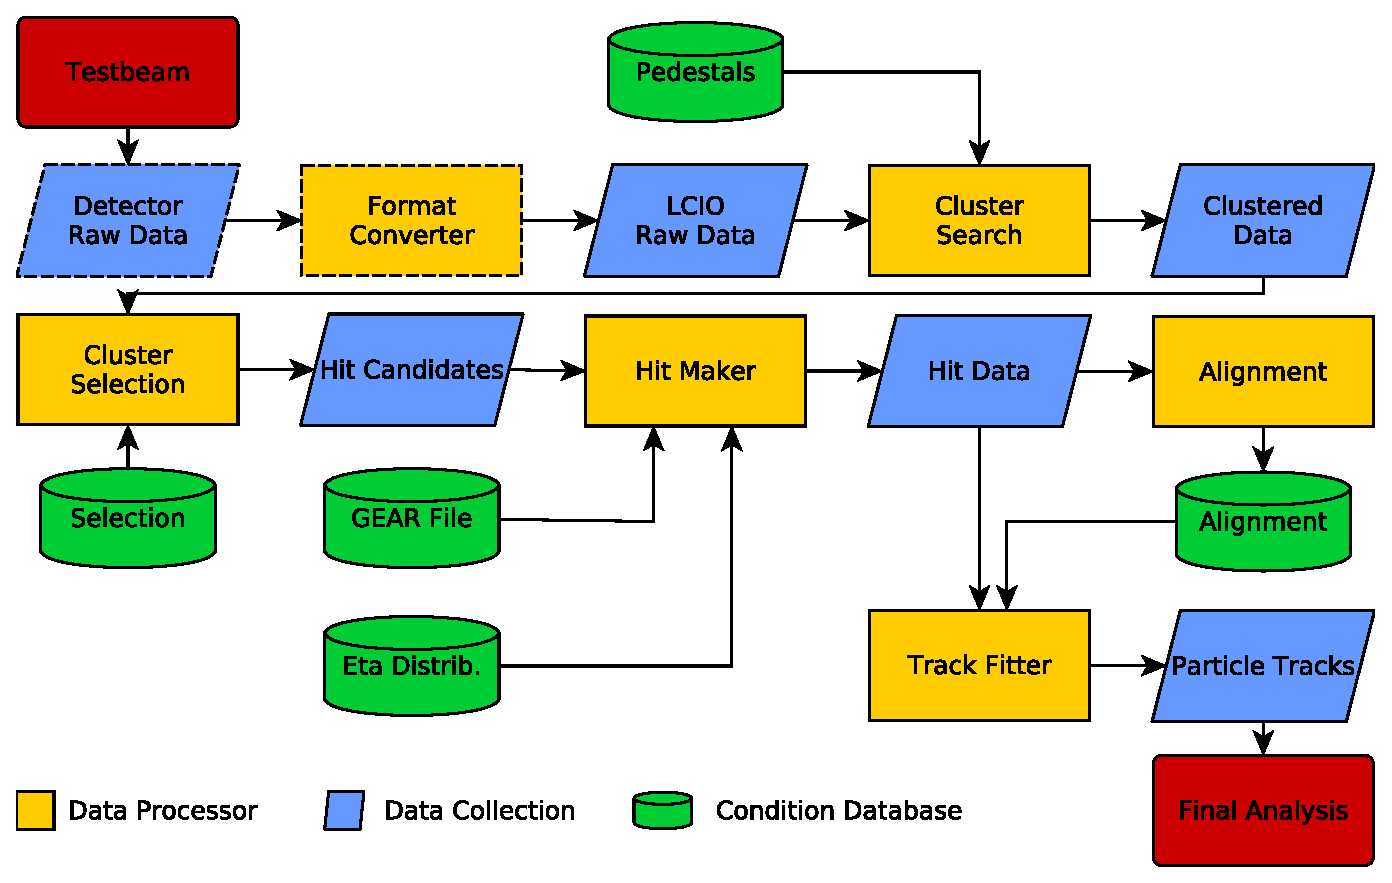
\includegraphics[width=.9\textwidth]{figures/eutel-strategy}
  \caption[The EUTelescope data analysis strategy]{Schematic of the overall telescope data reconstruction and analysis strategy of the EUTelescope framework.
EUTelescope provides processors for all steps, except for the conversion of the DUT raw data, marked with a dashed outline.}
  \label{fig:offline:strategy}
\end{figure}

EUTelescope provides several processors for Marlin, implementing algorithms necessary for a full track reconstruction and data analysis of test beam experiments. 
Figure~\ref{fig:offline:strategy} shows the analysis strategy of the framework starting from the recorded detector response to the final reconstructed particle tracks. 
%An overview of the processor range provided by EUTelescope is given in \cite{EUDET-2007-20}.
At low-energy beam lines such as the DESY-II test beam facility, multiple scattering is an important contribution to the overall track resolution uncertainty,
 especially in measurements with non-negligible DUT material budget, cf.\ section~\ref{sec:multiplescattering}.
Therefore, EUTelescope provides processors implementing advanced algorithms for tracking such as Deterministic Annealing Filter (DAF)~\cite{ref:daffitter}
 or GBL which account for scattering in all material present in the beam.
For high-energy beam lines a simple straight line fit provides sufficient precision and a maximum of computational performance.
In addition, precise offline detector alignment can be performed by minimising track residuals using the EUTelescope alignment processor which utilises the Millepede-II algorithm~\cite{Blobel-2006}.

EUTelescope comes with its own job submission framework Jobsub that allows to run analysis jobs on local machines or to submit them to larger computing clusters such as NAF for bulk reconstruction.
Using its flexible configuration file concept and the global run database storing user defined variables,
 jobsub eases the implementation of per-run variables for reconstruction such as beam energy or detector alignment.

 
The track parameters are calculated by employing a $\chi^{2}$-minimisation method~\cite{ref:eudetmemo_2007_01,ref:lutzpaper}.
For each telescope sensor dimension ($x$ and $y$), the individual contribution $\Delta \chi^2_{i}$ from plane $i$ is defined as

\begin{equation}
\label{eq:chi2contrib}
\Delta \chi^2_{i} = \left( \frac{r - p_{i}}{\sigmai} \right)^2 \Bigg|_{i \ne i_{\textrm{DUT}}} +
\left( \frac{\theta_{\textrm{i}} - \theta_{i-1}}{\Theta_{0}} \right)^2 \Bigg|_{i \ne 0,N-1} \,,
\end{equation}

\noindent
with the telescope plane numbering beginning at zero.
The measured hit position in one dimension is denoted by $r$, the position extrapolated from the track in the same dimension by $p_{i}$.
The angles between the nominal beam direction and the track direction are $\theta_{i-1}$ and $\theta_{i}$.
The former is the track angle entering plane $i$, the latter the angle of the outbound track segment.
The intrinsic resolution of sensor plane $i$ and the width of the multiple scattering distribution are denoted $\sigmai$ and $\Theta_{0}$, respectively, cf.~also section~\ref{sec:multiplescattering}. 
It is assumed that $\sigmai$ and $\Theta_{0}$ do not differ between planes and that $\sigmai$ is also equal for both measurement dimensions.
If the beam axis is denoted by $z$, then $\theta_i$ can be expressed as

\begin{equation}
\theta_i = \frac{p_{i+1} - p_i}{z_{i+1} - z_i} \,.
\end{equation}

\noindent In equation~(\ref{eq:chi2contrib}) the first term, resulting from the hit measurement, is excluded in the $\chi^2$ calculation if the considered plane is the DUT.
Similarly, for the first and last planes the second term in equation~(\ref{eq:chi2contrib}) is omitted, since the scattering angle can not be determined.
This results in the global $\chi^2$ expression

\begin{equation}
\label{eq:globalchi2}
\chi^2 = \sum_{i=0}^{N-1} \alpha_i \left( r - p_i \right)^2 + \sum_{i=1}^{N-2}
\left( \frac{p_{i + 1} \beta_i + p_{i-1} \beta_{i-1} - p_i \left( \beta_i + \beta_{i-1} \right)}{\Theta_0} \right)^2 \,,
\end{equation}

\noindent
with coefficients $\alpha_i$ and $\beta_i$ defined as~\cite{ref:eudetmemo_2007_01}

\begin{equation}
\alpha_i = \left\{
  \begin{array}{l l}
    \sigmai^{-2} & \quad \text{for $i \neq i_{\textrm{DUT}}$}\\
    0 & \quad \text{for $i = i_{\textrm{DUT}}$}
  \end{array} \right. \quad \text{and} \quad \beta_i = \frac{1}{z_{i + 1} - z_i} \,.
\end{equation}

\noindent
which is minimised with respect to the track parameters $p_i$. 


\section{Track Resolution}

\section{Conclusion}

\section*{Acknowledgement}

\small
\bibliographystyle{plain}
\bibliography{bibtex/refs}

\end{document}


